
\section{Curve Construction: Python Code}
\label{python_code}

Our curve construction code consists of four separate files for each of different methodologies. In order to reduce duplication, we present one full script for the method: \textit{Linear Interpolation of Explicit Discount Factors}, and then only a subsection of the remaining three scripts. The construction of the forward curve, using cubic spline interpolation, was identical for all four methodologies, hence, we only include the full script once. Python scripts that plot the curves have been omitted, but are available upon request.

\newpage

\subsection{Linear Interpolation of Explicit Discount Factors}

\begin{figure}[ht]
\begin{center}
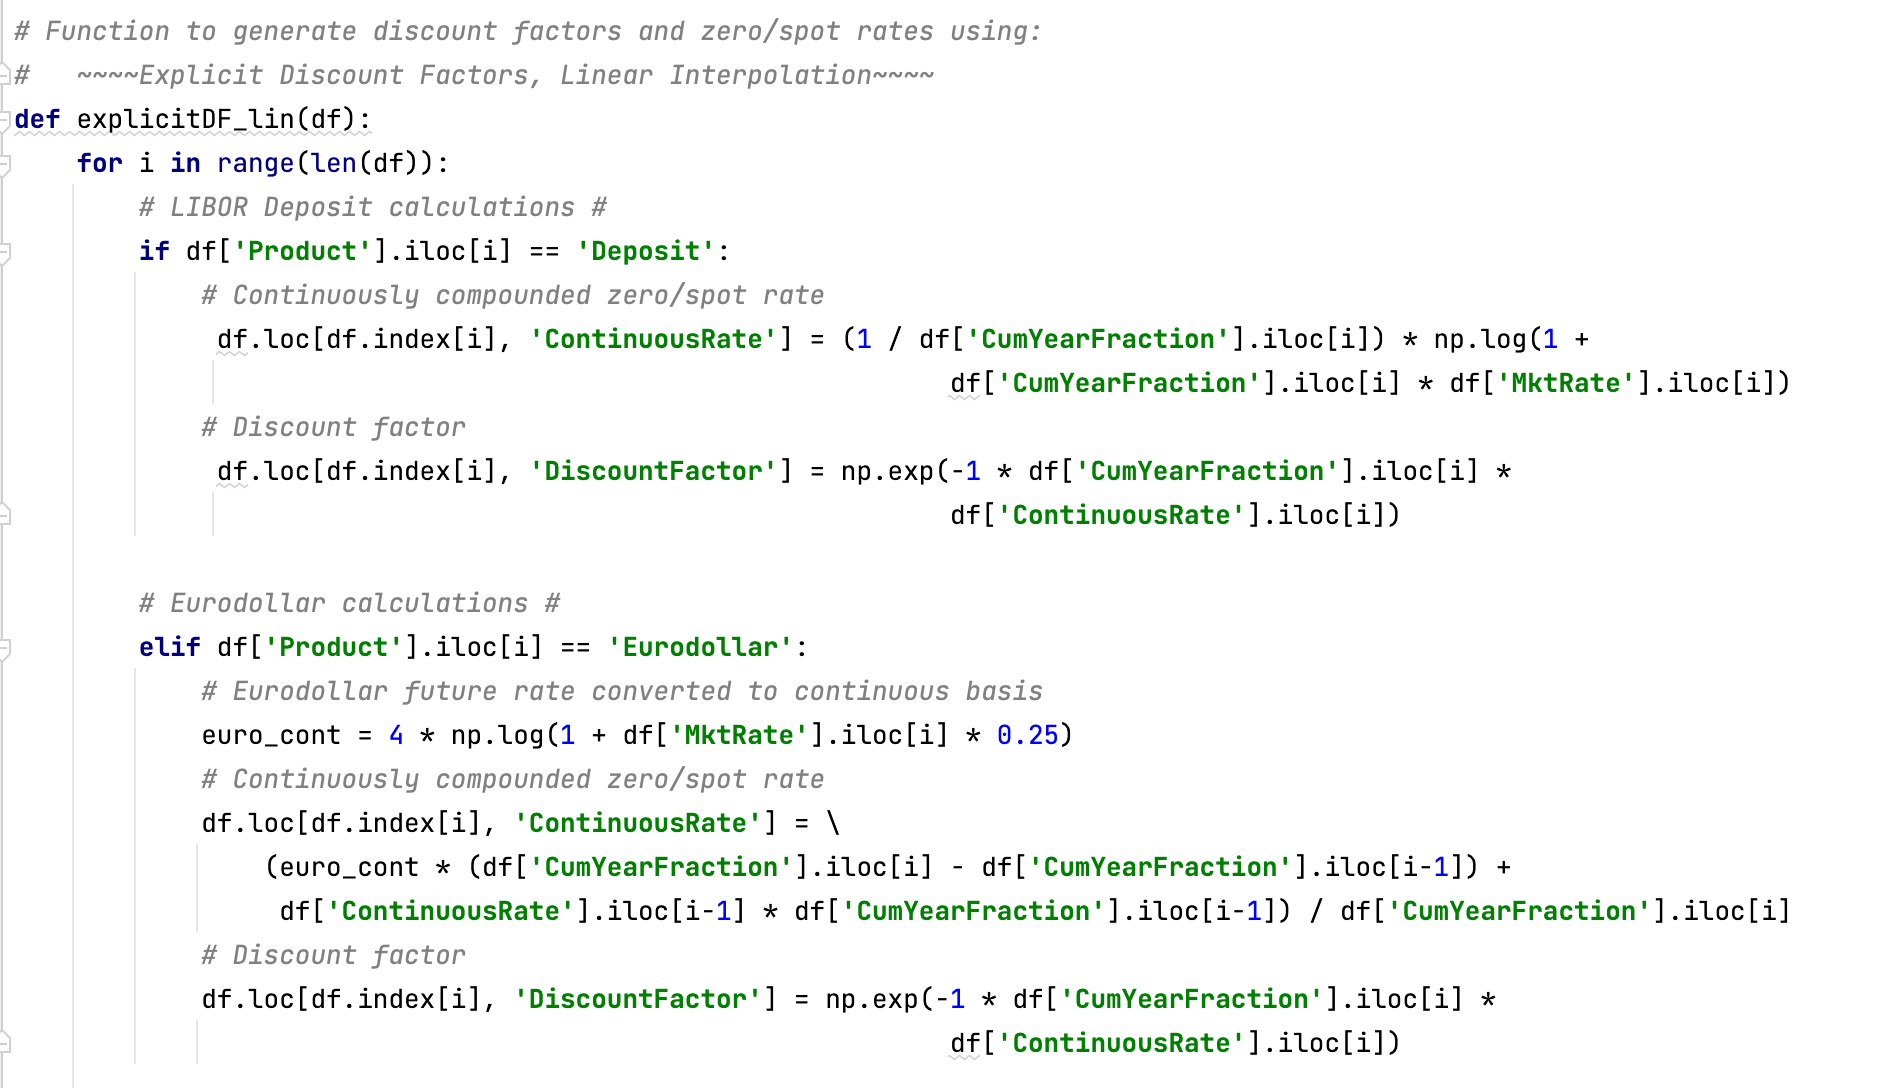
\includegraphics[width=0.99\textwidth]{Appendices/images/explicit_lin_function (1).png}
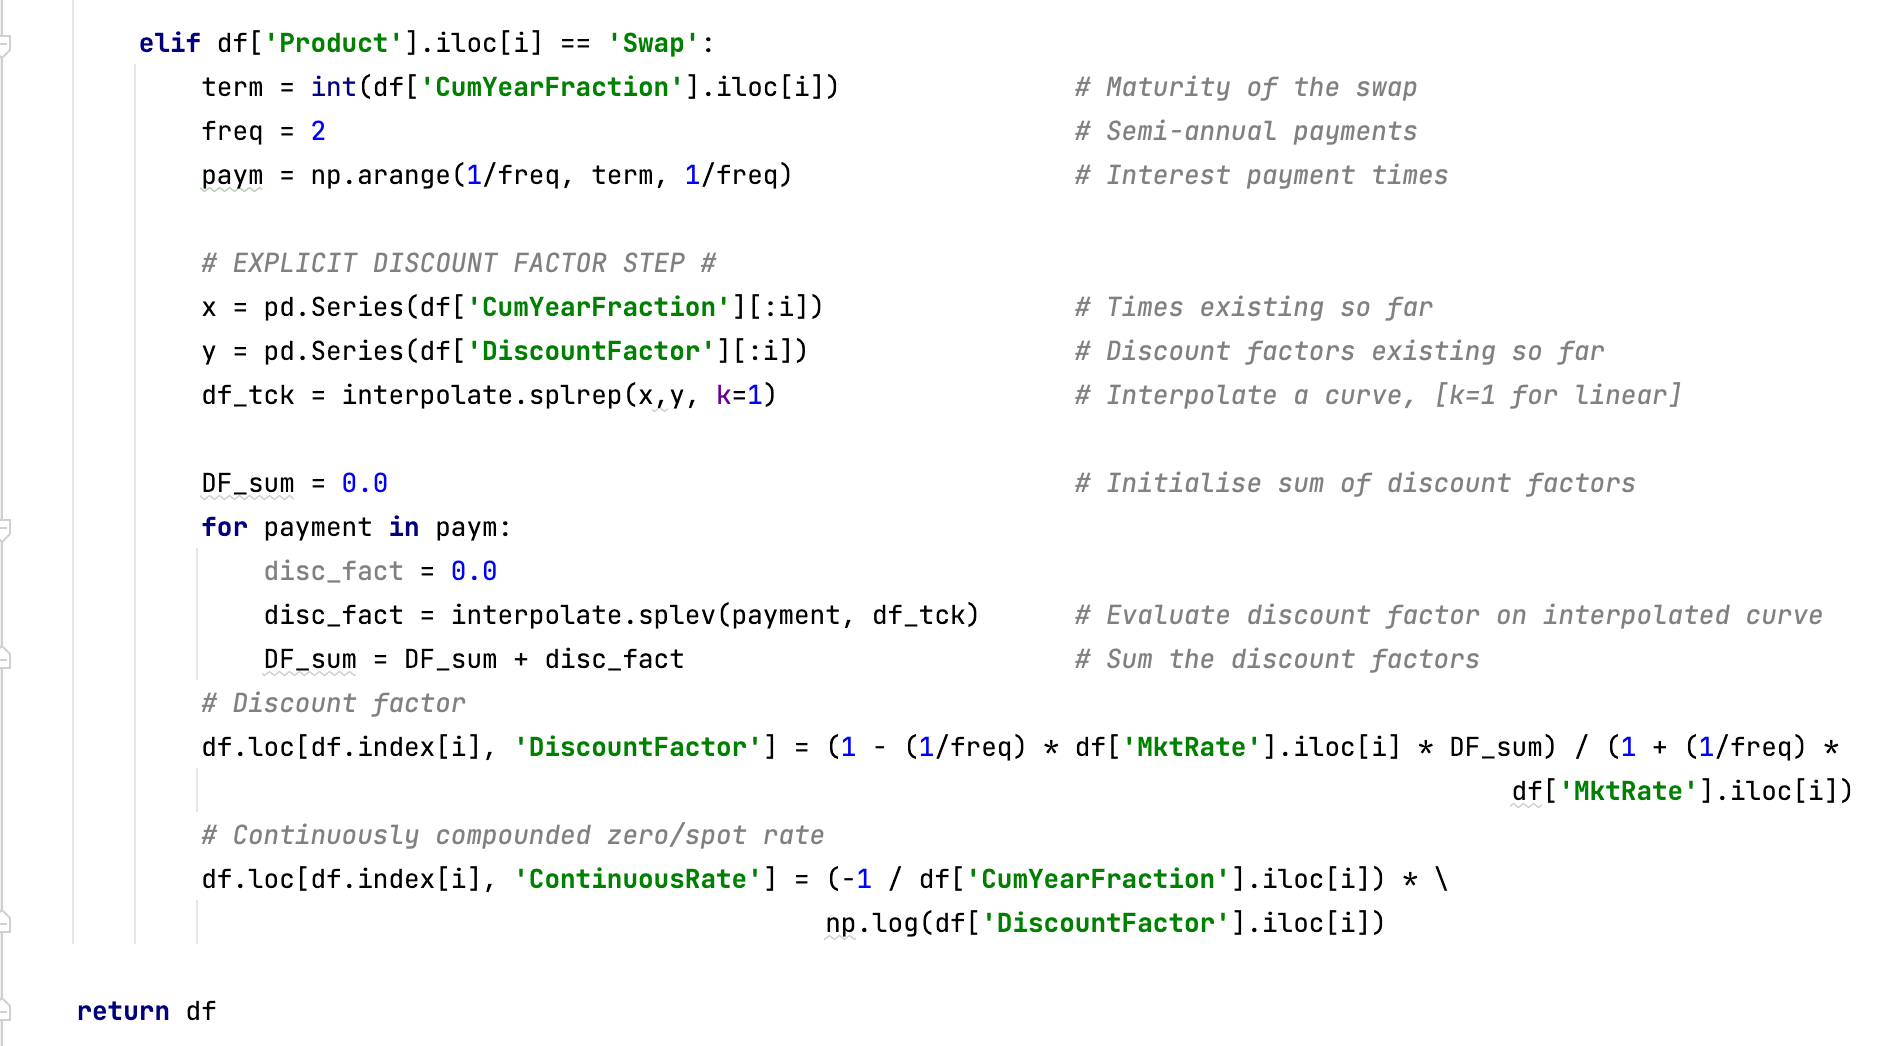
\includegraphics[width=0.99\textwidth]{Appendices/images/explicit_lin_function (2).png}
\end{center}
\end{figure}

\newpage

\subsection{Cubic Spline Interpolation of Explicit Discount Factors}

\begin{figure}[ht]
\begin{center}
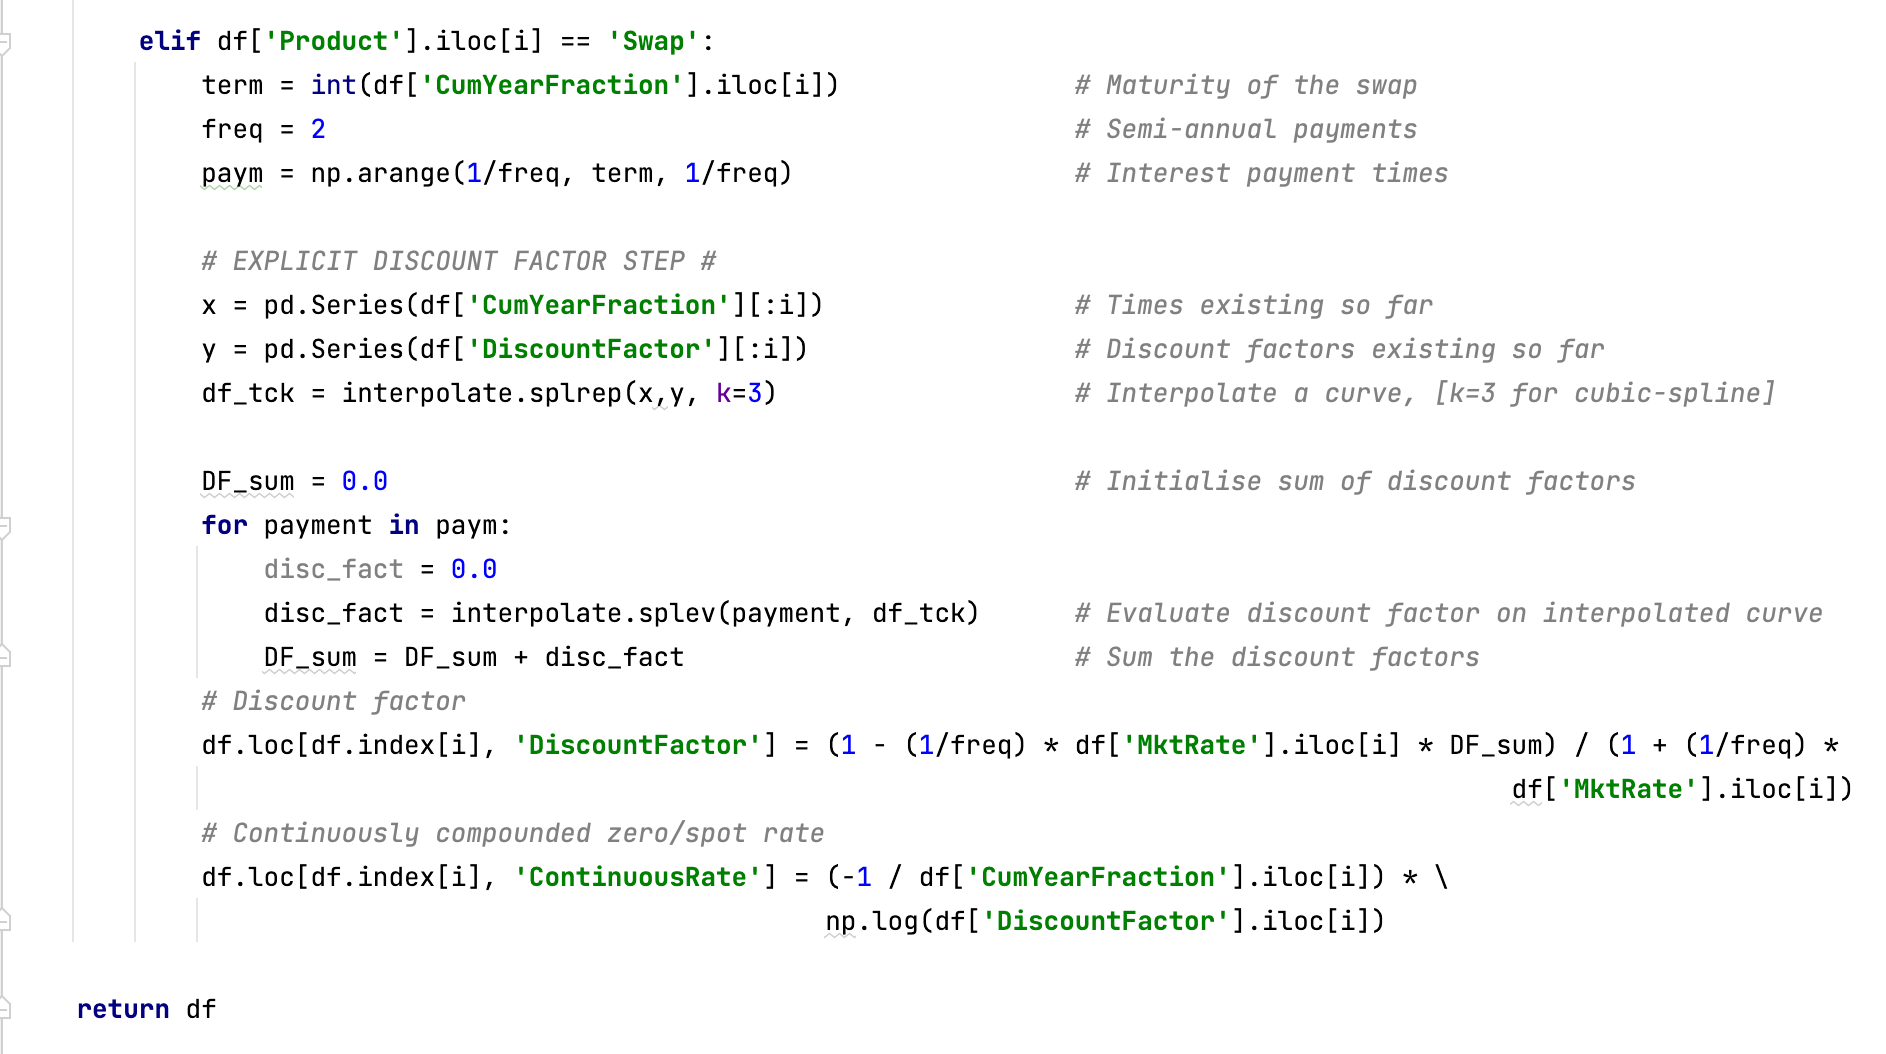
\includegraphics[width=0.99\textwidth]{Appendices/images/explicit_cube.png}
\end{center}
\end{figure}

\FloatBarrier

\subsection{Linear Spline Interpolation of Implicit Discount Factors}

\begin{figure}[ht]
\begin{center}
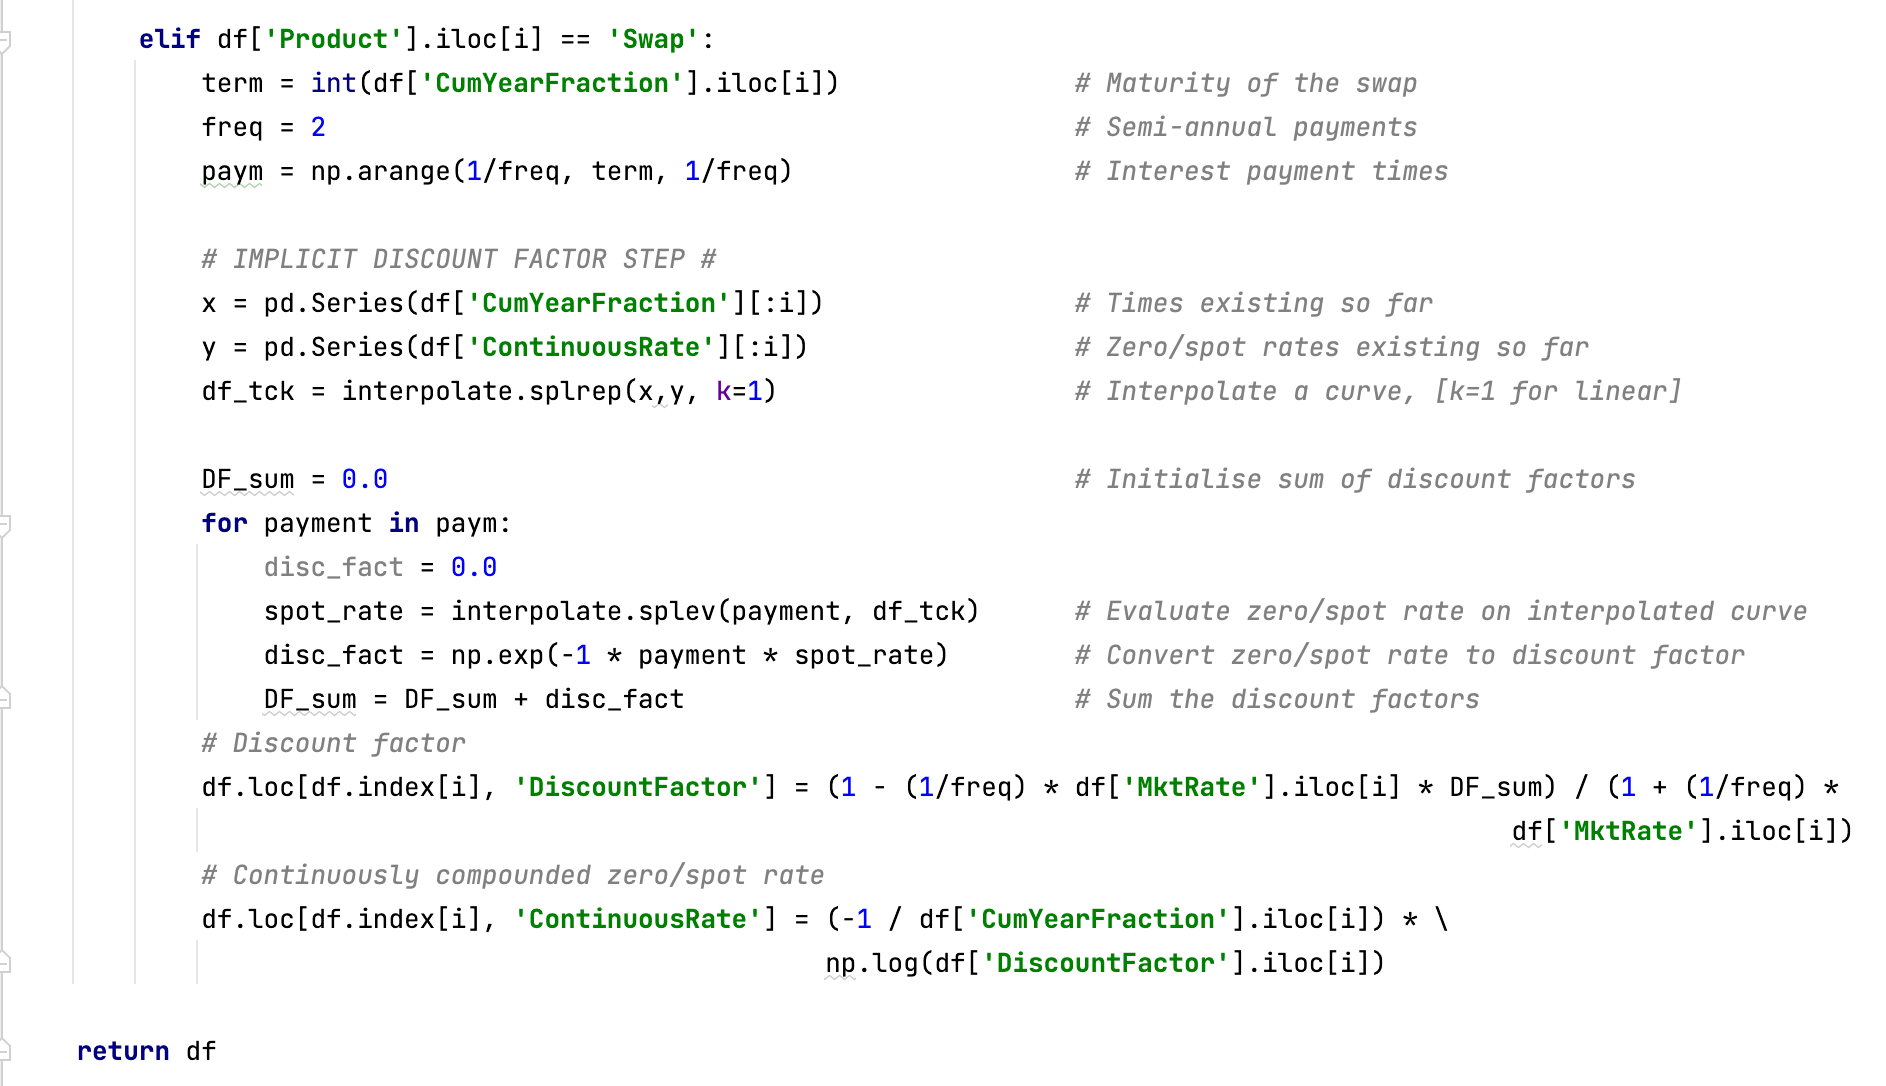
\includegraphics[width=0.99\textwidth]{Appendices/images/implicit_lin.png}
\end{center}
\end{figure}

\FloatBarrier

\newpage

\subsection{Cubic Spline Interpolation of Implicit Discount Factors}

\begin{figure}[ht]
\begin{center}
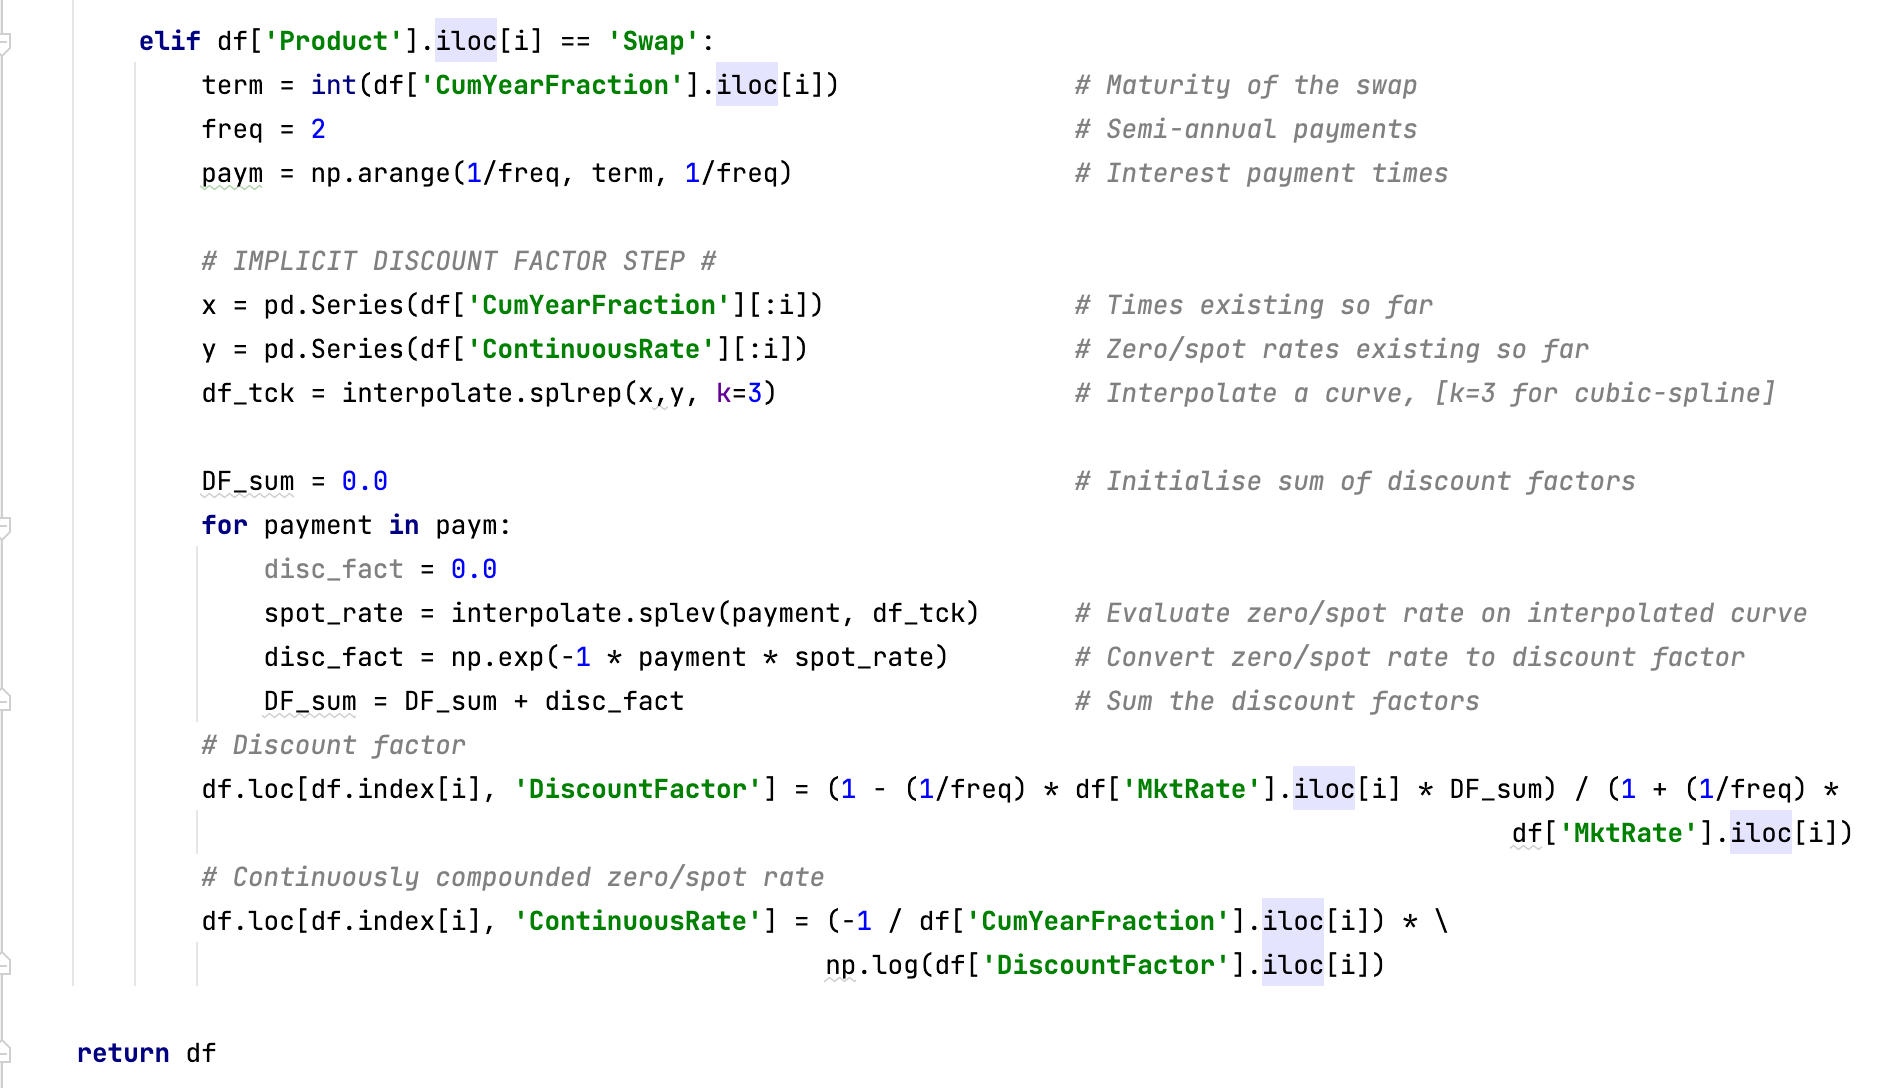
\includegraphics[width=0.99\textwidth]{Appendices/images/implicit_cube.png}
\end{center}
\end{figure}

\FloatBarrier

\subsection{Forward Curve}

\begin{figure}[ht]
\begin{center}
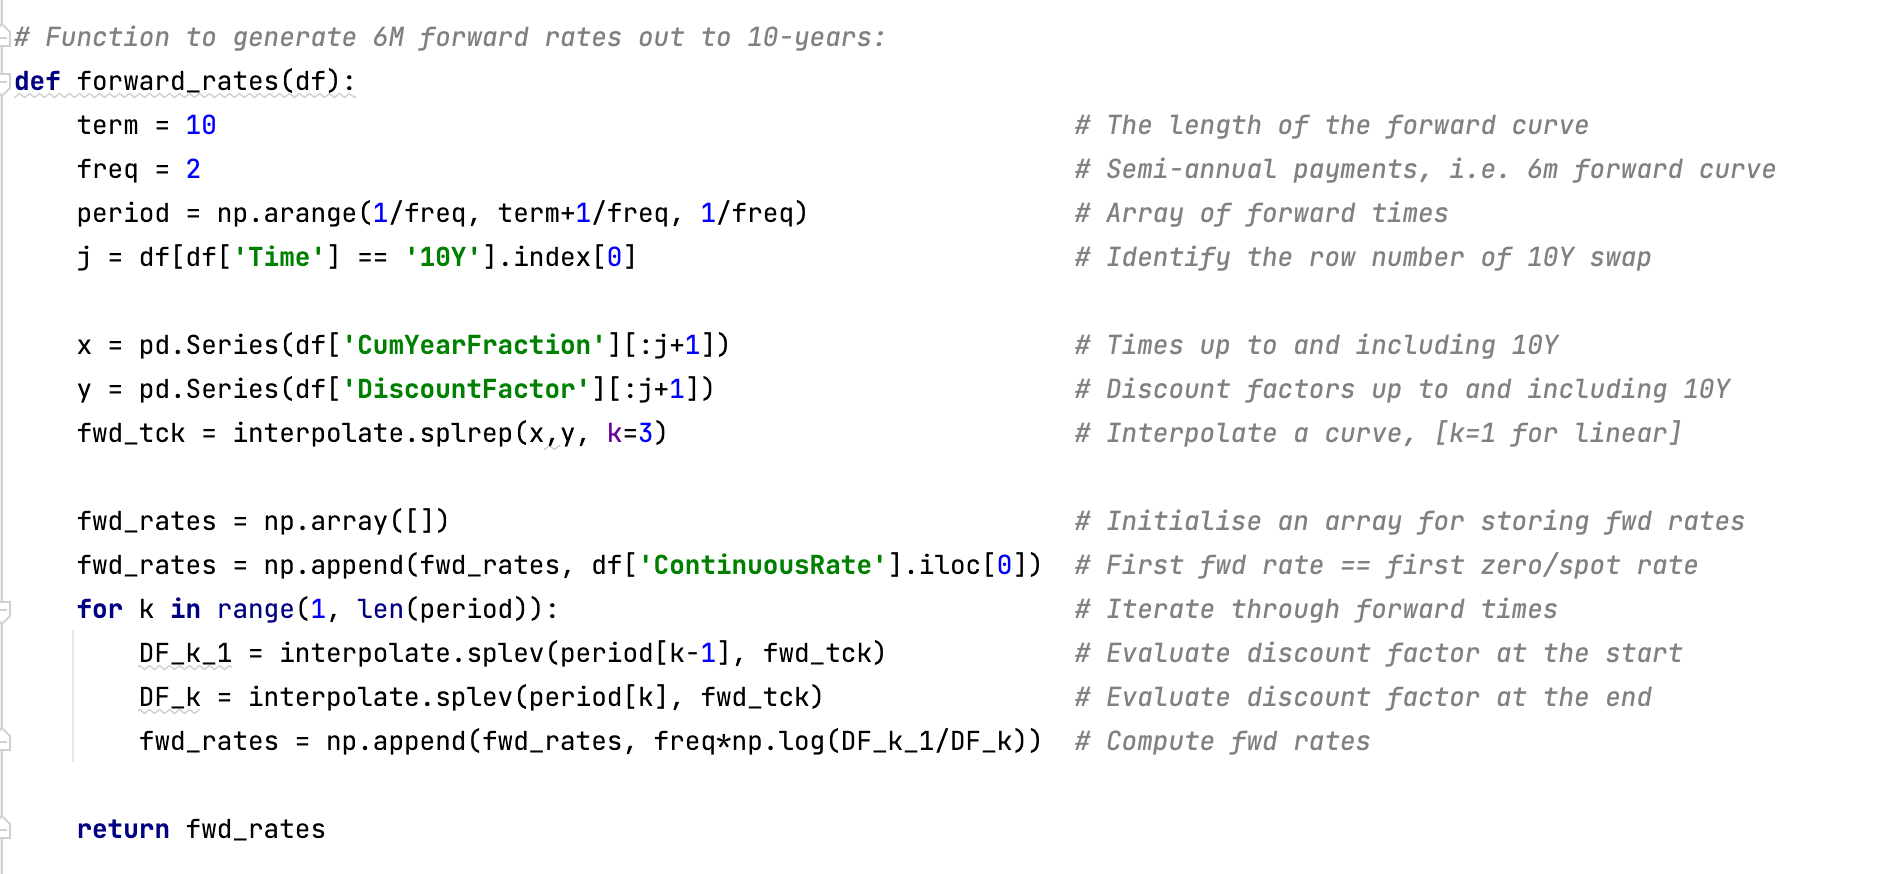
\includegraphics[width=0.99\textwidth]{Appendices/images/fwd_rate_function.png}
\end{center}
\end{figure}